% Compile with: latexmk -lualatex main.tex
\documentclass[11pt]{article}
\usepackage[review]{acl}
\usepackage{fontspec}
\setmainfont{TeX Gyre Termes}
\newfontfamily\arabicfont[Script=Arabic,Path=fonts/,Extension=.ttf,UprightFont=*-Regular,BoldFont=*-Bold]{Amiri}
\newcommand{\ar}[1]{\mbox{\textdir TRT\arabicfont #1}}
\usepackage{microtype}
\usepackage{enumitem}
\usepackage{amsmath,amssymb,amsthm,nicefrac,bm}
\usepackage{booktabs,multirow,siunitx}
\usepackage{graphicx,xcolor,colortbl}
\usepackage{tikz}
\usetikzlibrary{positioning,arrows.meta,calc}
\usepackage{pgfplots}
\pgfplotsset{compat=1.18}
\usepackage{algorithm}
\usepackage[noend]{algpseudocode}
\usepackage[capitalise,noabbrev]{cleveref}
\newtheorem{proposition}{Proposition}
\newcommand{\pending}[1]{\textcolor{red}{[PENDING: #1]}}

\title{SelectNorm: A Disagreement-Factorized Analysis of Per-Input\\ Normalization for Arabizi with Frozen Encoders}

\author{Anonymous submission}

\renewcommand{\dbltopfraction}{.95}\renewcommand{\dblfloatpagefraction}{.6}\renewcommand{\topfraction}{.9}\renewcommand{\floatpagefraction}{.6}\renewcommand{\textfraction}{.08}
\begin{document}
\maketitle
\begin{abstract}
A classifier trained on Arabic-script text can be applied to Latin-script Arabizi directly or after transliteration, and the better choice varies from input to input. We ask whether, with frozen encoders and linear heads, this choice can be learned per input and transferred from Tunisian to Algerian and Moroccan Arabizi, and, if not, why. We use an elementary identity: for binary labels the expected benefit of normalizing is the probability that the two views disagree times the margin by which the normalized view wins when they do. The identity separates disagreement detection, conditional advantage estimation and a cost-aware decision, so each can be measured on its own. With four frozen encoders, normalizing improves macro-F1 by 2--19 points on Tunisian and Algerian sets, and on Moroccan text its sign depends on the encoder. Learned per-input routing does not consistently exceed strong baselines or the better single view. Against a direct-gain router every paired 95\% interval lies within $\pm0.7$ points; against single views most intervals are inconclusive. Because routing must run the first pass before deciding, it costs more than either single view. The factorized analysis locates the limit for the features and estimators we test: disagreements are moderately predictable (AUC 0.62--0.74), but which view wins is weakly predictable from decision-point features (AUC at most 0.71, below 0.5 in two cases), also when a linear estimator is fitted on target labels. This is limited predictability under these choices, not unpredictability in principle. A bootstrap-classifier reference suggests that part of the oracle headroom is classifier variability. The usable signal is mostly set-level, which about a hundred labels recover.
\end{abstract}

\section{Introduction}
\label{sec:intro}

North African social-media text is written in Arabic script, in Latin-script Arabizi with digits standing for Arabic consonants (\textit{3}=\ar{ع}, \textit{7}=\ar{ح}), and with French segments inside the same sentence. A classifier trained on Arabic-script data can be applied to Arabizi in two ways: on the original string, or after transliterating it to Arabic script. Transliteration helps when it recovers words the classifier knows, and harms when it garbles French segments, negation, names or the spelling conventions of another dialect. The usual choice is made once for a whole dataset \citep{muller2021unseen,moosa2023transliteration,artetxe2023revisiting}, although the right choice varies from one input to the next.

This paper asks whether a frozen classifier can learn, without labels at inference time, \emph{for which inputs} normalization pays off, and whether that decision transfers from Tunisian to Algerian and Moroccan Arabizi. Learning a per-input benefit predictor is not new: post-hoc deferral rules estimate the gain of a second stage \citep{jitkrittum2023cascade}, and loss predictors choose test-time transformations \citep{kim2020learningloss}. What these methods do not address is how such a rule should be moved to a new dialect, where it is most likely to be wrong and where labels are scarce.

We start from an elementary identity. With binary labels, the expected benefit of normalizing an input equals the probability that the two views disagree, times the margin by which the normalized view wins when they do (\cref{eq:factor}). The first factor requires no labels; the second requires labels only on disagreements. The identity is not new in substance (it underlies disagreement-based methods such as query-by-committee), and we use it as an analysis device: it splits the routing problem into disagreement detection, conditional advantage estimation and a cost-aware decision, which can be estimated, adapted and \emph{measured} separately. We ask whether per-input selection beats dataset-level choices and strong routers (RQ1), across corpora and dialects (RQ2); what it costs (RQ3); whether normalized predictions agree with predictions on human transliterations (RQ4); which sub-problem limits it (RQ5); and how much a few target labels help (RQ6). All conclusions concern frozen encoders with linear heads. We contribute:
\begin{itemize}[leftmargin=1.2em,itemsep=0pt,topsep=2pt]
\item a disagreement-factorized analysis of selective normalization: a cost-aware Bayes rule that separates sunk from avoidable inference cost, and estimators and adaptation regimes for each factor, built from standard tools (\cref{sec:formulation,sec:method});
\item empirical evidence, across four frozen encoders and three Maghrebi varieties, on how far the \emph{conditional advantage} of a normalized view, the factor that per-input routing hinges on, can be predicted from decision-point features with linear and boosted estimators (\cref{sec:mechanism});
\item a controlled, pre-specified evaluation with latency-based costs checked by end-to-end timing, paired tests with multiplicity correction, and interval estimates for the mechanism measurements (\cref{sec:setup,sec:results});
\item a conservative Arabizi normalizer with safeguards for French segments, negation and non-lexical cues; its intrinsic scores are development results, not an independent test (\cref{tab:intrinsic}).
\end{itemize}
Normalization helps substantially on Tunisian and Algerian text, and its sign on Moroccan text depends on the encoder. SelectNorm stays within one point of the strongest router, but neither it nor any learned router consistently beats the better single view, and per-input routing is more expensive than either single view because the first pass is sunk. The analysis locates the limit in the conditional advantage: disagreements are moderately predictable, but the winning view is only weakly predictable from the features and estimators we test, even in domain. We report this rather than tune the method against the test sets.

\section{Related Work}
\label{sec:related}

\paragraph{Deferral, cascades and routing.}
Selective classification abstains when confidence is low \citep{geifman2017selective,geifman2019selectivenet}; learning to defer trains a classifier and a deferral rule jointly \citep{mozannar2020defer}. Closest to our setting are post-hoc cascade rules: \citet{jitkrittum2023cascade} show that confidence-based deferral is optimal only when the second stage's errors are uniform and propose estimating the gain of deferring directly, and \citet{gupta2024cascades} learn deferral from token-level uncertainty. LLM routers learn which model to query from preference data \citep{ong2025routellm} or from predicted weak--strong disagreement \citep{noorani2026disagreement}. These methods choose between \emph{models}; SelectNorm keeps one frozen model and chooses between two \emph{views} of the input. Its estimator differs from direct gain prediction by factorizing the gain into a label-free disagreement propensity and a label-dependent conditional win rate (\cref{eq:factor}), which determines what can be adapted without labels and where labels are informative.

\paragraph{Selecting input transformations.}
\citet{kim2020learningloss} predict, from the original image, the loss of each test-time augmentation and apply the best ones; our B4b baseline transfers this idea. \citet{kang2026luar} train an LLM with reinforcement learning to decide whether to translate a query before reasoning. Translate-test is usually chosen per task rather than per input \citep{artetxe2023revisiting}. None of these works studies the transfer of the selection rule across dialects.

\paragraph{Transliteration and dialect normalization.}
Transliterating unseen scripts can help multilingual encoders \citep{muller2021unseen,moosa2023transliteration}, and Arabizi has been converted to Arabic script with rules, lexicons and sequence models \citep{darwish2014arabizi,shazal2020unified}. Dialect normalization maps dialectal text to a standard variety with rules and LLMs \citep{dimakis2025dialect} or with dialect identification \citep{alhafni2024exploiting}, and DialUp adapts models to dialect continua and dialect data to models \citep{bafna2025dialup}; \citet{toughrai2025modeling} model North African dialects from standard languages. These approaches transform all inputs. SelectNorm treats the transformation as an action whose benefit is estimated per input and can be withheld.

\paragraph{Using disagreement without labels.}
Agreement between predictors has been used to estimate accuracy on unlabeled data \citep{platanios2014estimating,garg2022atc}, and querying labels where predictors disagree is the principle of query-by-committee \citep{seung1992qbc}. We use disagreement between two views of the same input to separate the label-free and label-dependent parts of a routing rule.

\section{Problem Formulation}
\label{sec:formulation}

\paragraph{Setting.}
Let $x$ be an input sentence with binary label $y\in\{0,1\}$, $T$ a deterministic normalizer that maps Latin-script Arabizi to Arabic script, and $f_\theta$ a frozen classifier with posterior $p_a=f_\theta(v_a)$ on view $v_0=x$ or $v_1=T(x)$ and decision $\hat y_a=\mathbf 1[p_a>\nicefrac12]$.
A routing policy $g:\mathcal Z\to\{0,1\}$ selects the view whose decision is returned, $\hat y(x)=\hat y_{g(z)}$, where $z=z(x)$ collects the features available at the \emph{decision point}: after $f_\theta(x)$ and $T(x)$ have been computed and before $f_\theta(T(x))$ is run.
Let $e_a=\mathbf 1[\hat y_a\neq y]$. Measured inference costs, relative to the mean cost of $f_\theta(x)$, are $c_0(x)$ for the first pass, $c_T(x)$ for the normalizer and $c_1(x)$ for the second pass $f_\theta(T(x))$. Because $z$ contains $p_0$ and normalizer metadata, $c_0+c_T$ is \emph{sunk} when $g$ is decided; only $c_1$ is \emph{avoidable}.

\paragraph{Objective and Bayes rule.}
For a trade-off $\lambda\ge0$ we seek
\begin{equation}
\min_g\;\mathbb E\big[e_{g(z)}+\lambda\,\big(c_0+c_T+c_1\,g(z)\big)\big].
\label{eq:risk}
\end{equation}
The sunk term does not depend on $g$, so conditioning on $z$ shows that the minimizer is
\begin{equation}
g^\star(z)=\mathbf 1\big[B(z)>\lambda\,\bar c(z)\big],
\label{eq:bayes}
\end{equation}
where $B(z)=\mathbb E[e_0-e_1\mid z]$
and $\bar c(z)=\mathbb E[c_1\mid z]$, the expected \emph{avoidable} cost. $B(z)$ is the expected \emph{benefit} of normalizing. The sunk cost matters when routing is compared with other systems: a router that reads $p_0$ and $m$ costs at least $c_0+c_T$, whereas never normalizing costs $c_0$ and always normalizing costs $c_T+c_1$. Per-input routing of this kind can therefore save compute only relative to running both views, never relative to a single view. It is the quantity estimated by post-hoc deferral rules \citep{jitkrittum2023cascade} and, for input transformations, by loss predictors \citep{kim2020learningloss}; estimating it directly is therefore not new.

\paragraph{Disagreement factorization (elementary).}
Let $D=\mathbf 1[\hat y_0\neq\hat y_1]$ and $W=\mathbf 1[\hat y_1=y]$.
Because $e_0=e_1$ whenever $D=0$, and because with binary labels exactly one view is correct whenever $D=1$,
\begin{align}
B(z)&=\pi(z)\,\big(2\rho(z)-1\big),\label{eq:factor}\\
\pi(z)&=P(D{=}1\mid z),\nonumber\\
\rho(z)&=P(W{=}1\mid D{=}1,z).\nonumber
\end{align}
(With $K$ classes, $B=\pi\,(\rho_1-\rho_0)$ with $\rho_a$ the probability that view $a$ is right given a disagreement.)
The identity is elementary and is implicit in disagreement-based methods such as query-by-committee \citep{seung1992qbc}; we do not claim it as a theoretical contribution. We use it as an \emph{analysis device}: the two factors have different data requirements and can be measured separately:
$\pi$ depends on the two views' predictions only, so it can be estimated on \emph{unlabeled} text once both views are run offline;
$\rho$ needs labels, but only on disagreements, since labels of agreeing inputs carry no information about $B$.

\paragraph{Three sub-problems.}
\Cref{eq:bayes,eq:factor} split selective normalization into \emph{disagreement detection} ($\pi$), \emph{conditional advantage estimation} ($\rho$) and a \emph{cost-aware decision} ($\lambda\bar c$). Both estimators are fitted by minimizing the log-loss, a proper scoring rule, on the policy split: $\hat\pi$ on all inputs with target $D$, $\hat\rho$ on disagreements with target $W$. The plug-in rule is $\hat g=\mathbf 1[\hat\pi(2\hat\rho-1)>\lambda\bar c]$. Two consequences follow directly.

\emph{(i) At zero cost the rule ignores $\pi$.} For $\lambda=0$ and $\hat\pi>0$, $\hat g=\mathbf 1[\hat\rho>\nicefrac12]$: the decision depends only on the conditional advantage, so re-estimating $\pi$ can change decisions only at $\lambda>0$.

\emph{(ii) Errors of each factor are weighted by the other.}
\begin{proposition}[Plug-in regret]
\label{prop:regret}
Let $R(g)$ be the risk in \cref{eq:risk}. Then
\[
R(\hat g)-R(g^\star)\le\mathbb E\big[\,|2\rho-1|\,|\hat\pi-\pi|+2\hat\pi\,|\hat\rho-\rho|\,\big].
\]
\end{proposition}
The usual plug-in argument gives $R(\hat g)-R(g^\star)\le\mathbb E|\hat B-B|$, and $\hat B-B=(\hat\pi-\pi)(2\rho-1)+2\hat\pi(\hat\rho-\rho)$ (\cref{app:proofs}). Errors in $\rho$ therefore cost most where disagreements are frequent. Errors in $\pi$ cost little when neither view dominates ($\rho\approx\nicefrac12$), which is also where any rule gains little. The bound is the standard plug-in argument applied to \cref{eq:factor} and is not a new learning-theoretic result; we use it only to motivate measuring the two estimation errors separately (\cref{sec:mechanism}).

\paragraph{Assumptions and limits.}
Exactness of \cref{eq:factor} requires binary labels and the 0-1 loss; macro-F1, our reported metric, is not a sum of per-input losses, so the rule is accuracy-optimal and only approximately macro-F1-optimal. Transfer of $\hat\rho$ to a new domain $Q$ assumes $P_Q(W\mid D{=}1,z)=P(W\mid D{=}1,z)$; this conditional invariance is the assumption we test.

\paragraph{Adaptation to a new dialect.}
A router trained on Tunisian data meets a target distribution $Q$ (another corpus or dialect). Re-estimating $\pi_Q$ on unlabeled target text is label-free; whether this suffices depends on the stability of $\rho$ across domains, which we test rather than assume (\S\ref{sec:results}).
When $\rho$ shifts, we model $\rho_Q(z)=\sigma\big(\operatorname{logit}\rho(z)+b\big)$ and estimate the scalar $b$ from $k$ labelled target disagreements.

\begin{proposition}[Label efficiency of disagreement-targeted labelling]
\label{prop:efficiency}
Under the model above, with $\pi_Q$ known, the Fisher information about $b$ carried by $k$ target labels drawn at random is $k\,P_Q(D{=}1)\,\mathbb E_Q[\rho_Q(1-\rho_Q)\mid D{=}1]$, and by $k$ labels drawn among disagreements it is $k\,\mathbb E_Q[\rho_Q(1-\rho_Q)\mid D{=}1]$. Targeted labelling is therefore $1/P_Q(D{=}1)$ times more informative.
\end{proposition}
The proof (\cref{app:proofs}) is a one-line Fisher-information calculation that uses only that an agreeing example's likelihood does not depend on $b$; it concerns the efficiency of estimating $b$, not the accuracy of the resulting router, which \cref{sec:results} tests. Labelling where predictors disagree is the idea of query-by-committee \citep{seung1992qbc}; here the target of estimation is a routing rule, and \cref{eq:factor} gives the exact reason why only disagreements matter.

\paragraph{Information access.}
The policy never reads $p_1$ at decision time; $\pi$ and $\rho$ are \emph{predicted} from $z$. Training uses $p_1$ on the policy split only, and adaptation uses $p_1$ on unlabeled target text that is disjoint from the evaluated fold. The oracle $g^{\rm or}=\mathbf 1[e_0{=}1\wedge e_1{=}0]$ reads labels and is reported only as an upper reference: ties and joint errors keep the original view at no cost.

\section{SelectNorm}
\label{sec:method}

\begin{figure*}[t]
\centering
% SelectNorm architecture (vector, TikZ). Top lane: inference path; bottom lane: fitted offline.
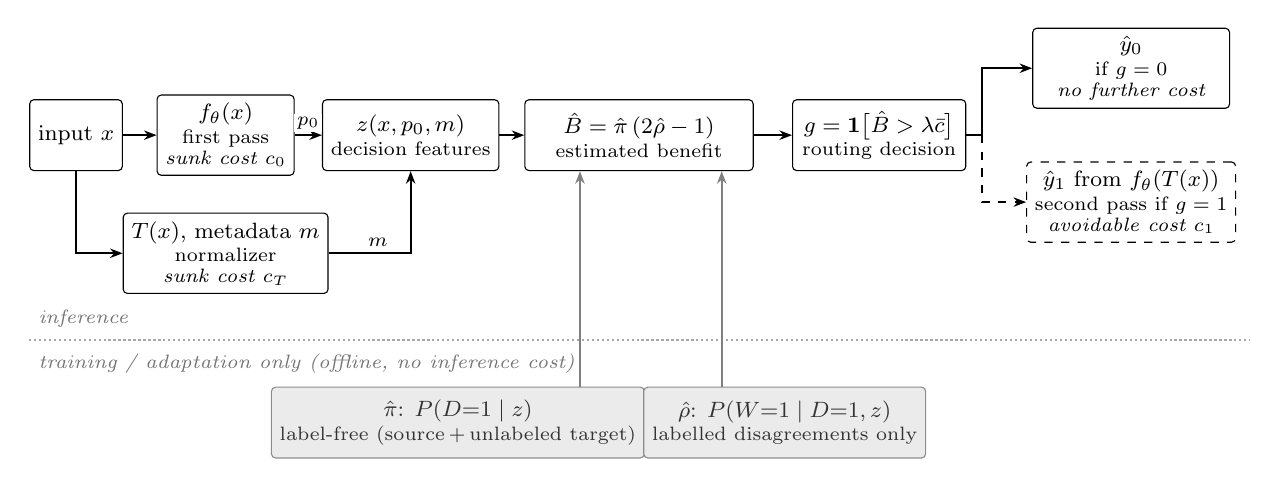
\begin{tikzpicture}[
  font=\footnotesize,
  box/.style={draw, rounded corners=1.5pt, align=center, minimum height=9mm, inner sep=3pt, fill=white},
  train/.style={box, fill=black!8, draw=black!45, text=black!80},
  arr/.style={-{Stealth[length=1.6mm]}, semithick},
  cond/.style={arr, dashed},
  lbl/.style={font=\scriptsize, fill=white, inner sep=1pt}]
% ---- inference lane ----
\node[box, minimum width=11mm] (x) at (0,0) {input $x$};
\node[box, minimum width=17mm] (f0) at (1.9,0) {$f_\theta(x)$\\[-1pt]\scriptsize first pass\\[-2pt]\scriptsize\itshape sunk cost $c_0$};
\node[box, minimum width=17mm] (T) at (1.9,-1.5) {$T(x)$, metadata $m$\\[-1pt]\scriptsize normalizer\\[-2pt]\scriptsize\itshape sunk cost $c_T$};
\node[box, minimum width=19mm] (z) at (4.25,0) {$z(x,p_0,m)$\\[-1pt]\scriptsize decision features};
\node[box, minimum width=29mm] (B) at (7.15,0) {$\hat B=\hat\pi\,(2\hat\rho-1)$\\[-1pt]\scriptsize estimated benefit};
\node[box, minimum width=22mm] (g) at (10.2,0) {$g=\mathbf 1\big[\hat B>\lambda\bar c\big]$\\[-1pt]\scriptsize routing decision};
\node[box, minimum width=25mm] (y0) at (13.4,0.85) {$\hat y_0$\\[-1pt]\scriptsize if $g=0$\\[-2pt]\scriptsize\itshape no further cost};
\node[box, minimum width=25mm, dashed] (f1) at (13.4,-0.85) {$\hat y_1$ from $f_\theta(T(x))$\\[-1pt]\scriptsize second pass if $g=1$\\[-2pt]\scriptsize\itshape avoidable cost $c_1$};
\draw[arr] (x) -- (f0);
\draw[arr] (x) |- (T);
\draw[arr] (f0) -- node[lbl, above=1pt]{$p_0$} (z);
\draw[arr] (T.east) -| node[lbl, pos=.3, above=1pt]{$m$} (z.south);
\draw[arr] (z) -- (B);
\draw[arr] (B) -- (g);
\coordinate (split) at ($(g.east)+(0.2,0)$);
\draw[semithick] (g.east) -- (split);
\draw[arr] (split) |- (y0.west);
\draw[cond] (split) |- (f1.west);
% ---- lane separator ----
\draw[black!35, densely dotted, thick] (-0.6,-2.6) -- (14.9,-2.6);
\node[anchor=south west, font=\scriptsize\itshape, text=black!55] at (-0.6,-2.57) {inference};
\node[anchor=north west, font=\scriptsize\itshape, text=black!55] at (-0.6,-2.65) {training / adaptation only (offline, no inference cost)};
% ---- training lane ----
\node[train, minimum width=33mm] (pi) at (4.85,-3.65) {$\hat\pi$: $P(D{=}1\mid z)$\\[-1pt]\scriptsize label-free (source\,+\,unlabeled target)};
\node[train, minimum width=33mm] (rho) at (9.0,-3.65) {$\hat\rho$: $P(W{=}1\mid D{=}1,z)$\\[-1pt]\scriptsize labelled disagreements only};
\draw[arr, black!50] (6.4,0 |- pi.north) -- (6.4,0 |- B.south);
\draw[arr, black!50] (8.2,0 |- rho.north) -- (8.2,0 |- B.south);
\end{tikzpicture}

\caption{SelectNorm. Top lane, inference: $f_\theta(x)$ and $T(x)$ always run, so their cost is sunk when $g$ is decided; the second pass $f_\theta(T(x))$ (dashed) is the only avoidable cost and runs only when the estimated benefit exceeds $\lambda\bar c$. Bottom lane, grey: estimators fitted offline for training or adaptation, with no inference cost beyond evaluating $\hat\pi,\hat\rho$.}
\label{fig:arch}
\end{figure*}

\paragraph{Module A: conservative normalizer.}
$T$ processes Latin-script tokens and leaves Arabic-script tokens, digits-only tokens, emoji and punctuation unchanged (\cref{alg:norm}).
A token is first looked up in a lexicon of Arabizi$\to$CODA pairs built from 80\% of TArC \citep{gugliotta2022tarc}; unseen tokens fall back to Tunisian character rules (\textit{3}$\to$\ar{ع}, \textit{7}$\to$\ar{ح}, \textit{9}$\to$\ar{ق}, \textit{5}$\to$\ar{خ}, \textit{ch}$\to$\ar{ش}, word-initial vowels to alef, medial short vowels dropped).
Three safeguards define $T_{\rm cons}$:
(i) \emph{protection} of French and English tokens, decided from word frequencies against TArC evidence, with short or function-like tokens (\textit{la}, \textit{ma}, \textit{el}) read in the language of their sentence context;
(ii) \emph{negation}: the Tunisian circumfix \textit{ma\ldots ch} is split as \ar{ما} + stem + \ar{ش} and frequent negators (\textit{mouch}, \textit{mech}) are mapped by a fixed list, so that the negation particle survives;
(iii) \emph{non-lexical cues}: laughter (\textit{hhhh}, \textit{mdr}) is mapped to \ar{ههه} rather than transliterated letter by letter.
Two weaker strategies serve as controls: $T_{\rm rule}$ (rules only) and $T_{\rm lex}$ (lexicon and rules, no safeguards).
Every call returns token-level reliability metadata (lexicon hits, rule fallbacks, ambiguous characters, protected, negation and laughter tokens), which the router may read because it is computed before the second pass.

\paragraph{Module B: benefit estimation.}
The decision-point features $z$ form three groups:
\emph{conf} (maximum probability, margin and entropy of the temperature-scaled $p_0$),
\emph{script} (length, Latin share, digits used as letters, emoji and upper-case rates),
and \emph{trel} (the normalizer metadata as rates per Latin token, and the share of changed tokens).
$\hat\pi$ and $\hat\rho$ are logistic regressions on standardized $z$ (gradient boosting as ablation); $\hat\rho$ is fitted on the disagreements of the policy split only (\cref{alg:train}).

\paragraph{Module C: cost-aware routing.}
At inference (\cref{alg:infer}) the classifier runs once on $x$, the normalizer runs (both costs are sunk at the decision point), and $\hat B(z)=\hat\pi(z)(2\hat\rho(z)-1)$ is compared with a threshold: either $\lambda\bar c$, the Bayes threshold of \cref{eq:bayes}, or, as for every baseline, a threshold tuned for each $\lambda$ on the policy development split. No threshold is tuned on target data. The second pass runs only when $g=1$; its cost $\bar c$ is the only avoidable cost, and it is the only cost that enters the threshold. Reported costs count everything a system runs (\cref{sec:setup}).

\paragraph{Complexity.}
Let $C_f(n)$ be the cost of one encoder pass on $n$ subword tokens. $T$ is $O(n)$ with dictionary lookups; $\hat\pi,\hat\rho$ cost $O(|z|)$. Expected inference cost is $C_f+C_T+O(|z|)+\mathbb E[g]\,C_f$, of which only the last term is avoidable; training the router costs one pass of each view over the policy split and $O(N|z|)$ per logistic fit. Adaptation adds one offline pass of each view over unlabeled target text and $k$ annotations.

\begin{algorithm}[t]
\small
\caption{Conservative normalization $T_{\rm cons}$}
\label{alg:norm}
\begin{algorithmic}[1]
\Require sentence $x$, lexicon $\mathcal L$, rules $R$, frequency lists $F$
\Ensure $T(x)$, metadata $m$
\State $\tau\gets$ tokens of $x$; $\kappa\gets$ share of foreign tokens in $\tau$ by $F$ vs.\ $\mathcal L$
\For{each Latin-script token $t\in\tau$}
  \If{$t$ is laughter} emit \ar{ههه}
  \ElsIf{$t$ is foreign (short: iff $\kappa>\nicefrac12$)} keep $t$
  \ElsIf{$t$ is a listed negator} emit its fixed form
  \ElsIf{$t\in\mathcal L$} emit $\mathcal L(t)$
  \ElsIf{$t$ matches \textit{ma\ldots ch}} emit \ar{ما} $R(\text{stem})$\ar{ش}
  \Else\ emit $R(t)$ and count ambiguous characters
  \EndIf
  \State update $m$ with the branch taken
\EndFor
\State \Return joined output, $m$
\end{algorithmic}
\end{algorithm}

\begin{algorithm}[t]
\small
\caption{Training (labels from the policy split only)}
\label{alg:train}
\begin{algorithmic}[1]
\Require frozen $f$, normalizer $T$, policy split $\mathcal P=\{(x_i,y_i)\}$; optional unlabeled target set $\mathcal U$; optional $k$ labelled target disagreements $\mathcal K$
\Ensure $\hat\pi$, $\hat\rho$ (and shift $\hat b$)
\For{$x\in\mathcal P\cup\mathcal U$} compute $p_0,p_1$, $z$, $D$ \EndFor
\State $\hat\rho\gets$ fit $P(W{=}1\mid z)$ on $\{i\in\mathcal P: D_i=1\}$ \Comment{needs $y$}
\State $\hat\pi\gets$ fit $P(D{=}1\mid z)$ on $\mathcal P$, or on $\mathcal P\cup\mathcal U$ with equal total weight \Comment{label-free}
\If{$\mathcal K\neq\emptyset$} \Comment{few-label shift (\cref{sec:formulation})}
  \State $\hat b\gets\arg\max_b \sum_{i\in\mathcal K}\log\mathrm{Bern}\big(W_i;\,\sigma(r_i+b)\big)-\tfrac{b^2}{2}$, \ $r_i=\operatorname{logit}\hat\rho(z_i)$
\EndIf
\end{algorithmic}
\end{algorithm}

\begin{algorithm}[t]
\small
\caption{Inference}
\label{alg:infer}
\begin{algorithmic}[1]
\Require input $x$, $f$, $T$, $\hat\pi$, $\hat\rho$, $\lambda$, mean avoidable cost $\bar c$ of $f(T(x))$
\Ensure label $\hat y$, action $g$, score $\hat B$
\State $p_0\gets f(x)$; $(x',m)\gets T(x)$; $z\gets z(x,p_0,m)$
\State $\hat B\gets\hat\pi(z)\,(2\hat\rho(z)-1)$; $g\gets\mathbf 1[\hat B>\lambda\bar c]$
\If{$g=1$} $\hat y\gets\mathbf 1[f(x')>\nicefrac12]$ \Comment{second pass}
\Else\ $\hat y\gets\mathbf 1[p_0>\nicefrac12]$ \EndIf
\State \Return $\hat y,g,\hat B$
\end{algorithmic}
\end{algorithm}

\section{Experimental Setup}
\label{sec:setup}

\begin{table}[t]
\centering\small
\setlength{\tabcolsep}{3pt}
\begin{tabular}{@{}llrrl@{}}
\toprule
Set & Variety, script & $N$ & Pos.\% & Role\\
\midrule
TSAC-\textsc{ar} & Tun., Arabic & 5{,}564 & 45.0 & $f$ (90/10)\\
TSAC-\textsc{lat} tr. & Tun., Latin & 6{,}204 & 57.3 & policy\\\\
\midrule
$S_3$ TSAC-\textsc{lat} & Tun., Latin & 1{,}425 & 55.2 & test\\
$S_4$ TUNIZI & Tun., Latin & 2{,}875 & 48.8 & test\\
$S_5$ NArabizi & Alg., Latin & 729 & 52.0 & test\\
$S_5^{\textsc{ar}}$ NArabizi gold & Alg., Arabic & 729 & 52.0 & RQ4\\
$S_6$ MYC-\textsc{lat} & Mor., Latin & 4{,}191 & 66.4 & test\\
\bottomrule
\end{tabular}
\caption{Data after de-duplication and near-copy removal (character 3-gram cosine $\ge0.9$ against every training or policy sentence). $S_5^{\textsc{ar}}$ is the human Arabic-script transliteration of $S_5$ \citep{touileb2021interplay}.}
\label{tab:data}
\end{table}

\paragraph{Data.}
\Cref{tab:data} lists the sets. The classifier is trained on Arabic-script TSAC \citep{medhaffar2017tsac}; the human Latin-script TSAC training comments, never seen by $f$, form the policy pool. Test sets cover the same corpus ($S_3$), another Tunisian corpus and platform ($S_4$, TUNIZI; \citealp{fourati2021tunizi}), Algerian ($S_5$, NArabizi; \citealp{seddah2020narabizi,touileb2021interplay}) and Moroccan Arabizi ($S_6$, MYC; \citealp{jbel2023myc}). Mixed-script sentences (minority alphabet $>20\%$ of letters) are excluded. Each row is its own resampling unit except the $S_5$/$S_5^{\textsc{ar}}$ pairs, which share a source identifier. Corpora were cloned at fixed commits and are not redistributed (\cref{app:repro}).

\paragraph{Classifiers.}
$f_\theta$ is a logistic regression on mean-pooled, frozen representations of four encoders: XLM-R base \citep{conneau2020xlmr}, mE5 base \citep{wang2024me5}, LaBSE \citep{feng2022labse} and MARBERTv2 \citep{abdulmageed2021marbert}, pinned to fixed revisions. The regularization constant is chosen and a temperature is fitted \citep{guo2017calibration} on the 10\% Arabic-script development split. No encoder is fine-tuned, and no Latin-script sentence is used to train $f$.

\paragraph{Systems.}
B0 keeps $x$; B1 always normalizes with $T_{\rm cons}$; B2 routes at random at SelectNorm's selection rate (20 draws); B3 thresholds the confidence of $p_0$; B4 estimates $B(z)$ directly as $P(\text{help}\mid z)-P(\text{harm}\mid z)$, a post-hoc deferral rule \citep{jitkrittum2023cascade}; B4b predicts each view's error \citep{kim2020learningloss}; B6 is the oracle; R averages both views' probabilities (always two passes). SelectNorm-src uses \cref{eq:factor} with source estimates; SelectNorm-adapt re-estimates $\hat\pi$ on unlabeled target text with two-fold cross-fitting by source sentence. All thresholds, including SelectNorm's, are tuned on the policy development split for each $\lambda$ (the protocol's primary variant); SelectNorm with the untuned Bayes threshold $\lambda\bar c$ is reported as a variant. Nothing is tuned on a test set.

\paragraph{Classifier regimes.}
In the primary regime $f$ sees only Arabic script. As an exploratory second regime, logged as a deviation before it was run, $f$ is also trained on a synthetic Latin rendering $G(x)$ of each training sentence, produced by inverting the TArC lexicon and the digit rules (\textsc{+syn}); this makes both views in-distribution to some degree and tests whether routing matters more when neither view dominates.

\paragraph{Few-label setting.}
This setting uses target labels and is reported separately. Each test set is split into two folds by source sentence. To predict fold $f$, a budget of $k\in\{8,16,32,64,128\}$ labels is drawn from the \emph{other} fold only, either at random or among its disagreements ($D$ is label-free); the labels re-estimate the shift $b$ of $\hat\rho$ (SelectNorm), re-fit B4's heads, re-tune B3, or choose B0 or B1 for the whole fold (set-level choice). No sentence is scored by a system that saw its label; an audit that replays every targeted and random draw, checked against the indices logged by a rerun, found no sentence whose own label informed its prediction (\cref{app:repro}). On $S_5$ at $k{=}128$ a fold has only 97--116 disagreements, so the targeted budget is smaller there. Each $k$ uses 5 draws $\times$ 5 seeds; all few-label systems use the $\lambda=0$ threshold, and the zero-shot reference is SelectNorm-adapt with the same threshold.

\paragraph{Mechanism analysis.}
To locate failures we measure four quantities separately for each encoder and test set (\cref{sec:mechanism}): (M1) how well $\hat\pi$ ranks disagreements (AUC; source-trained and label-free target cross-fitted); (M2) how well $\hat\rho$ ranks the winning view among disagreements (AUC), its calibration gap, and a diagnostic ceiling obtained by cross-validating $\hat\rho$ on \emph{target} labels (5 folds; not deployable); (M3) the macro-F1 gain over the best single view of the $\lambda{=}0$ rule $\hat\rho>\nicefrac12$ under both estimates; (M4) the oracle headroom, compared with a \emph{reference}: the headroom between two classifiers trained on bootstrap resamples of the same data and applied to the same original input. The reference shows how large ``choose whichever is right'' gains can be from training-sample variability alone; it is a diagnostic, not a decomposition of the headroom, and we report its sensitivity (\cref{tab:noise}). Test labels serve only as evaluation targets. Intervals for M1--M3 are 95\% percentile intervals from 1{,}000 bootstrap resamples of test sentences; each resample reweights all five seeds' predictions with the same counts and averages over seeds, so repeated measurements are not treated as independent; estimators are not refitted, so the intervals cover evaluation sampling only.

\paragraph{Metrics and statistics.}
Macro-F1 is primary; we also report accuracy, selection rate, harmful transformations (a correct original prediction made wrong) per 100 inputs, the share of oracle opportunities captured, and inference cost relative to one pass of $f$ on $x$, charging each system for what it runs (estimated from a token-length model fitted to measured latencies, and checked by end-to-end timing; \cref{app:repro}) (\cref{fig:pareto}). Results average five seeds. $f$ is trained once per encoder and regime; seed $s$ fixes the policy split (hence routers and thresholds), B2's draws and the few-label draws. Fits are deterministic, so seed variation reflects the policy split only, not retraining of $f$. Differences are tested with a paired bootstrap over source sentences \citep{koehn2004bootstrap,dror2018hitchhiker} (10{,}000 resamples, seed-averaged statistic), with Holm correction over all main comparisons of an encoder. We call a difference practically relevant only if it is at least one macro-F1 point and significant after correction (the protocol's wording requires only the unadjusted interval to exclude zero; the two coincide in the primary regime, and for \textsc{+syn} we report both). A non-significant difference is not read as equivalence; where we say two systems perform alike, we give the paired difference and its interval (\cref{tab:paired}).

\paragraph{Status of analyses.} Pre-specified in the protocol (\cref{app:repro}): main comparisons and statistics, the $\lambda$ grid, the embedding, boosting and $T_{\rm lex}$ ablations, the few-label setting and RQ4; other ablations use the pre-registered code but are not named in it. Exploratory, logged after the first mE5 results: $T_{\rm cov}$, \textsc{+syn} and M1--M4. Added in revision: intervals, sensitivity and equivalence readings, end-to-end timing, the normalizer audit and the input-dependent cost threshold.

\section{Results}
\label{sec:results}

\begin{table*}[t]
\centering\small\setlength{\tabcolsep}{4.5pt}
\begin{tabular}{@{}lrrrrrrrr@{}}\toprule
 & \multicolumn{4}{c}{\textbf{mE5}} & \multicolumn{4}{c}{\textbf{XLM-R}}\\
\cmidrule(lr){2-5}\cmidrule(lr){6-9}
 & $S_3$ & $S_4$ & $S_5$ & $S_6$ & $S_3$ & $S_4$ & $S_5$ & $S_6$\\\midrule
B0 original & 63.4$^{\triangledown}$ & 61.5$^{\triangledown}$ & 63.6$^{\triangledown}$ & \textbf{54.1} & 54.5$^{\triangledown}$ & 48.8$^{\triangledown}$ & 48.6$^{\triangledown}$ & 63.5$^{\triangledown}$\\
B1 always normalize & \textbf{82.0} & \textbf{67.2} & 69.4 & 52.9 & 72.8 & \textbf{64.5} & 63.1 & 72.3$^{\blacktriangle}$\\
B2 random, matched rate & 80.0 & 66.5 & 68.5 & 53.2 & 70.2 & 63.3 & 61.9 & 68.9\\
B3 confidence threshold & 82.0 & 67.2 & 69.4 & 52.9 & 72.9 & 64.4 & 63.0 & \textbf{72.3}$^{\blacktriangle}$\\
B4 direct gain & 81.4 & 67.0 & 69.9 & 53.6 & 73.5 & 63.9 & 63.3 & 68.7\\
B4b per-view loss & 81.6 & 67.1 & 69.9 & 53.7 & \textbf{73.9} & 63.9 & \textbf{63.4} & 68.2\\
SelectNorm-src & 81.3 & 67.0 & \textbf{70.0} & 53.7 & 73.8 & 63.8 & 63.4$^{\blacktriangle}$ & 68.0$^{\triangledown}$\\
\rowcolor{black!6}SelectNorm-adapt & 81.3 & 66.9 & 69.8 & 53.7 & 73.8 & 63.8 & 63.1 & 68.5\\
\quad Bayes threshold $\lambda\bar c$ & 81.4 & 66.9 & 69.6 & 53.5 & 73.9 & 64.0 & 63.4 & 69.0\\
\addlinespace[2pt]
R two-view ensemble$^\dagger$ & 78.9 & 66.5 & 69.7 & 54.4 & 67.3 & 57.2 & 54.7 & 69.7\\
B6 oracle$^\ddagger$ & 90.0 & 81.3 & 81.8 & 63.8 & 83.1 & 75.2 & 70.4 & 82.1\\
\midrule[\heavyrulewidth]
 & \multicolumn{4}{c}{\textbf{LaBSE}} & \multicolumn{4}{c}{\textbf{MARBERTv2}}\\
\cmidrule(lr){2-5}\cmidrule(lr){6-9}
 & $S_3$ & $S_4$ & $S_5$ & $S_6$ & $S_3$ & $S_4$ & $S_5$ & $S_6$\\\midrule
B0 original & 69.6$^{\triangledown}$ & 61.1$^{\triangledown}$ & 65.6$^{\triangledown}$ & \textbf{63.4}$^{\blacktriangle}$ & 64.3$^{\triangledown}$ & 62.4$^{\triangledown}$ & 60.0 & 52.5$^{\triangledown}$\\
B1 always normalize & 83.6 & \textbf{69.1} & 70.9 & 55.5$^{\triangledown}$ & 82.1 & 67.7 & 62.3 & 58.3\\
B2 random, matched rate & 81.0 & 67.3 & 69.5 & 60.4 & 79.9 & 67.3 & 61.9 & 56.7\\
B3 confidence threshold & 83.7 & 69.1 & 70.9 & 55.9$^{\triangledown}$ & \textbf{82.3} & 68.1 & 62.3 & \textbf{58.3}\\
B4 direct gain & 83.4 & 68.6 & 71.6 & 60.6 & 82.1 & 68.2 & \textbf{63.0} & 57.6\\
B4b per-view loss & 83.3 & 68.9 & \textbf{71.6} & 60.5 & 82.1 & 68.1 & 62.8 & 57.6\\
SelectNorm-src & 83.4 & 68.7 & 71.1 & 60.4$^{\triangledown}$ & 82.2 & 68.3 & 62.9 & 57.7\\
\rowcolor{black!6}SelectNorm-adapt & 83.4 & 68.8 & 71.5 & 60.9 & 82.1 & \textbf{68.3} & 62.9 & 57.7\\
\quad Bayes threshold $\lambda\bar c$ & \textbf{83.7} & 68.8 & 71.3 & 60.8 & 82.2 & 68.1 & 62.5 & 57.9\\
\addlinespace[2pt]
R two-view ensemble$^\dagger$ & 81.7 & 68.4 & 72.1 & 60.5 & 82.3 & 69.7 & 62.4 & 58.4\\
B6 oracle$^\ddagger$ & 91.5 & 82.2 & 85.7 & 75.2 & 93.6 & 84.2 & 77.6 & 70.4\\
\bottomrule\end{tabular}

\caption{Macro-F1 ($\lambda=0$, mean of five seeds), classifier trained on Arabic script only; two encoders per panel. Bold: best deployable system per column. Shaded: SelectNorm-adapt, the protocol's primary system. $^{\triangledown}$/$^{\blacktriangle}$: the baseline is significantly worse/better than SelectNorm-adapt (paired bootstrap, Holm-corrected $p<0.05$ over the protocol's 20 comparisons per encoder; tested only for B0, B1, B3, B4 and SelectNorm-src). R always runs both passes; B6 uses test labels.}
\label{tab:main}
\end{table*}

\subsection{Selective normalization against strong baselines (RQ1, RQ2)}
\label{sec:main-results}
\Cref{tab:main} gives the main comparison. Normalization itself matters: always normalizing (B1) improves over the original input on the three Tunisian and Algerian sets for every encoder, by 2.3 to 18.6 macro-F1 points. On Moroccan MYC the sign depends on the encoder: B1 gains 8.8 points with XLM-R and loses 7.9 with LaBSE.

Learned routing does not add a consistent improvement on top of this. Against the direct-gain router B4 no difference is significant, and every 95\% interval lies inside $[-0.63,+0.58]$, i.e.\ within the protocol's 1-point relevance margin in all 16 cells (an equivalence reading added post hoc; \cref{tab:paired}). SelectNorm-adapt and -src differ by $-0.25$ to $+0.54$ points (three small differences are significant), and all learned routers are descriptively within about one point of each other. Against B1 and B3, SelectNorm-adapt is relevantly better in one cell (LaBSE on MYC, $+5.5$ and $+5.0$), where normalizing is harmful and confidence thresholding fails to stop it, and relevantly worse in one (XLM-R on MYC, $-3.8$), where normalizing is right and the router keeps the original view for about 40\% of inputs; in the LaBSE MYC cell it is also relevantly worse than B0, the better view there ($-2.5$). Elsewhere, non-significance is not equivalence: only 4 (B1) and 6 (B3) of the 16 intervals lie within $\pm1$ point, and the other non-significant ones extend from $-1.3$ to $+2.4$, so a small gain or loss cannot be excluded. Under the decision rule fixed for this study, SelectNorm therefore shows no consistent, statistically supported gain over competitive baselines; the rest of this section analyses why.

\subsection{Accuracy and cost (RQ3)}
\begin{figure*}[t]
\centering
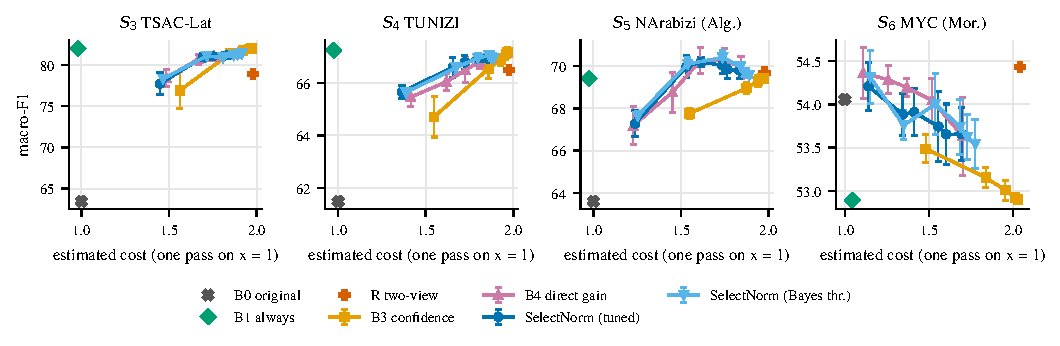
\includegraphics[width=\textwidth]{figures/pareto.pdf}
\caption{Macro-F1 against estimated inference cost (mE5, batch size 1, CPU; one pass of $f$ on $x$ = 1; per-sentence encoder costs from a token-length model fitted to measured latencies, see \cref{app:repro}), for $\lambda\in\{0,.01,.02,.05,.1,.2\}$; error bars: s.d.\ over seeds. Each system is charged for what it runs: B0 one pass on $x$; B1 the normalizer and one pass on $T(x)$; learned routers the first pass and the normalizer (sunk) plus the second pass when selected; B3 the first pass plus normalizer and second pass when selected; R both passes.}
\label{fig:pareto}
\end{figure*}
Each single-view system runs one encoder pass: B0 costs 1.00 and B1 0.97--1.04 passes on $x$ (the normalizer adds about 0.4\%). A router that decides from $p_0$ has already paid for the first pass: at $\lambda=0$, SelectNorm-adapt costs 1.69--1.88 passes for mE5 and 1.43--1.88 across encoders, against 1.89--2.05 for the two-view ensemble. Raising $\lambda$ lowers the cost (to 1.14--1.45 for mE5 at $\lambda=0.2$), but macro-F1 falls towards that of B0 (\cref{fig:pareto}). Per-input routing of this kind is thus never cheaper than the better single view and, never being relevantly more accurate (at most $+0.6$ points, not significant), offers no accuracy--cost advantage over it; it saves compute only relative to running both views. Thresholding with each input's own avoidable cost instead of the mean only moves points along the same frontier. These costs are token-model estimates; running the deployed pipeline end to end, with live routing decisions that reproduce the archived ones exactly, gives the same picture (B1 0.91--1.05, SelectNorm-adapt 1.31--1.97, R 1.91--2.07 passes; \cref{app:repro}). Descriptively, B4 and B3 trace similar curves, and the untuned Bayes threshold a curve close to that of tuned thresholds.

\subsection{Where per-input routing fails (RQ5)}
\label{sec:mechanism}
\begin{table*}[t]
\centering\footnotesize\setlength{\tabcolsep}{3.2pt}
\resizebox{\textwidth}{!}{\begin{tabular}{@{}llrrrrrrrrrr@{}}\toprule
 & & \multicolumn{2}{c}{(M1) disagreement} & \multicolumn{4}{c}{(M2) direction} & \multicolumn{2}{c}{(M3) benefit} & \multicolumn{2}{c}{(M4) headroom}\\
\cmidrule(lr){3-4}\cmidrule(lr){5-8}\cmidrule(lr){9-10}\cmidrule(lr){11-12}
Enc. & Set & $P(D)$ & AUC$_\pi$ & $P(W|D)$ & AUC$_\rho$ & AUC$_\rho^{\rm tgt}$ & gap & $\Delta_{\rm src}$ & $\Delta_{\rm tgt}$ & oracle & vs.\ ref.\\\midrule
mE5 & $S_3$ & 34 & 0.68 & 77 & 0.66 & 0.64 & +3 & -0.6$^{*}$ & +0.0 & 8.0 & -0.3\\
 & $S_4$ & 33 & 0.64 & 57 & 0.56 & 0.58 & +19$^{*}$ & -0.3 & -0.1 & 14.1 & +4.6\\
 & $S_5$ & 29 & 0.62 & 58 & 0.63 & 0.57$^\circ$ & +15$^{*}$ & +0.2 & +0.7 & 12.4 & +3.2\\
 & $S_6$ & 21 & 0.74 & 47 & 0.54 & 0.56 & +20$^{*}$ & -0.5 & +0.2 & 9.7 & +4.6\\
\midrule
XLM-R & $S_3$ & 36 & 0.64 & 72 & 0.71 & 0.68 & +3 & +1.0$^{*}$ & +0.8 & 10.3 & +5.9\\
 & $S_4$ & 31 & 0.66 & 64 & 0.57 & 0.57 & +11$^{*}$ & -0.5 & +0.3 & 10.7 & +7.6\\
 & $S_5$ & 23 & 0.69 & 69 & 0.45$^\circ$ & 0.60$^\circ$ & +11$^{*}$ & +0.3 & -0.7 & 7.3 & +2.1\\
 & $S_6$ & 28 & 0.72 & 69 & 0.44 & 0.66 & -8$^{*}$ & -3.3$^{*}$ & +1.1$^{*}$ & 9.8 & +4.5\\
\midrule
LaBSE & $S_3$ & 30 & 0.69 & 73 & 0.61 & 0.53$^\circ$ & -0 & +0.1 & -0.1 & 7.9 & +1.3\\
 & $S_4$ & 34 & 0.65 & 62 & 0.57 & 0.59 & +6$^{*}$ & -0.4 & -0.4 & 13.0 & +5.7\\
 & $S_5$ & 34 & 0.65 & 58 & 0.59 & 0.55$^\circ$ & +3 & +0.4 & +0.2 & 14.9 & +7.5\\
 & $S_6$ & 31 & 0.68 & 33 & 0.57 & 0.64 & +16$^{*}$ & -2.6$^{*}$ & +0.8$^{*}$ & 11.8 & +5.3\\
\midrule
MARBERTv2 & $S_3$ & 39 & 0.69 & 70 & 0.63 & 0.60 & +1 & +0.1 & -0.3 & 11.5 & +0.8\\
 & $S_4$ & 37 & 0.71 & 60 & 0.61 & 0.64 & +13$^{*}$ & +0.4 & +2.8$^{*}$ & 16.5 & +2.0\\
 & $S_5$ & 31 & 0.73 & 57 & 0.63 & 0.54$^\circ$ & +13$^{*}$ & +0.2 & +1.1 & 15.3 & +3.6\\
 & $S_6$ & 30 & 0.71 & 59 & 0.55 & 0.63 & +4$^{*}$ & -0.3 & +1.1$^{*}$ & 12.1 & -0.7\\
\bottomrule\end{tabular}
}
\caption{The four mechanisms of \cref{sec:formulation} ($T_{\rm cons}$, Arabic-script classifier, mean of five seeds). (M1) disagreement rate (\%) and AUC of label-free, target-cross-fitted $\hat\pi$. (M2) win rate of $T(x)$ on disagreements (\%), AUC of source-trained $\hat\rho$, AUC of a diagnostic $\hat\rho$ cross-validated on target labels (not deployable), and calibration gap of source $\hat\rho$ (points). (M3) macro-F1 gain over the best single view of the rule $\hat\rho>\nicefrac12$ with source and with target-CV $\hat\rho$. (M4) oracle headroom over the best view, and the same minus the headroom between two bootstrap-resampled classifiers on the same input (a diagnostic reference, not a decomposition; see \cref{tab:noise}). $^\circ$: the 95\% interval of the AUC contains 0.5; $^{*}$: the interval of the gap or gain excludes 0 (1{,}000 seed-averaged bootstrap resamples; all intervals in \cref{tab:mechanism-ci}). Test labels are used for analysis only.}
\label{tab:mechanism}
\end{table*}
The factorization lets us measure each sub-problem separately (\cref{tab:mechanism}).

\paragraph{(M1) Disagreement is moderately predictable.} Between 21\% and 39\% of inputs change label under normalization, and the label-free estimate ranks them with AUC 0.62--0.74; every 95\% interval lies between 0.57 and 0.77 (\cref{tab:mechanism-ci}). Re-estimating $\hat\pi$ on unlabeled target text raises this AUC most on MYC (for mE5 from 0.67 with source training to 0.74), but the Bayes rule at $\lambda=0$ depends on $\hat\rho$ alone (\cref{sec:formulation}); accordingly SelectNorm-src and -adapt differ by at most about half a point at $\lambda=0$.

\paragraph{(M2) Direction is weakly predictable from $z$, even in domain.} Which view is right when they disagree is ranked by source-trained $\hat\rho$ with AUC 0.54--0.71 in 14 of 16 cells (interval upper bounds at most 0.76); for XLM-R on Algerian text the interval includes 0.5, and on Moroccan text it lies below it ($[0.41,0.48]$). Fitting $\hat\rho$ on target labels by cross-validation, an upper reference that no deployable system has, reaches 0.53--0.68 (upper bounds at most 0.73), and its interval includes 0.5 in five cells. With linear estimators, the decision-point features thus carry little information about direction in any domain we tested; this does not exclude that other features or estimators would predict it better. What does change across domains is the \emph{level} of $\rho$: the win rate ranges from 33\% to 77\% across encoder--set pairs, and source $\hat\rho$ is miscalibrated out of domain, with gaps whose intervals exclude zero in 11 of 12 out-of-domain cells (up to $+20$ points).

\paragraph{(M3) The expected benefit follows.} The rule $\hat\rho>\nicefrac12$ gains between $-3.3$ and $+1.0$ points over the best single view with source estimates; only one gain has an interval above zero (XLM-R, $S_3$, $+1.0$), and three losses lie below zero. With the target-CV ceiling the change is $-0.7$ to $+2.8$, with interval upper bounds of at most $+3.9$. Most of the gap between routing and the oracle is therefore not a transfer problem: with these features and a linear estimator, it remains when the router is fitted on the target.

\paragraph{(M4) A reference for the oracle headroom.} The oracle gains 7--17 points over the best view, which looks like large headroom. Two classifiers that differ only in a bootstrap resample of their training data, applied to the same input, show 3--15 points of the same kind of headroom without any normalization. This reference is a diagnostic, not a decomposition: it depends strongly on how the two classifiers are made (2--6 points with 80\% subsamples, 5--22 points with weaker regularization; \cref{tab:noise}), so it cannot say how much of the views' headroom is recoverable. It does show that oracle headroom of this size arises from training-sample variability alone, and that oracle headroom is a weak indicator of what a router can gain.

\paragraph{Linguistic conditions.} On the Tunisian and Algerian sets, always normalizing helps less on inputs with many French or English tokens or low lexicon coverage, for every encoder but one case (XLM-R, TUNIZI, French/English) (\cref{tab:taxonomy}); negation and length show no consistent pattern. On MYC the net effect of every condition has a different sign for different encoders, so the main determinant of whether normalization pays there is the encoder--dialect pair, not a property of the input that $z$ could observe.

\begin{table*}[t]
\centering\footnotesize\setlength{\tabcolsep}{4pt}
\begin{tabular}{@{}lrrrr@{}}\toprule
Condition (share of $S_3$/$S_4$/$S_5$/$S_6$) & $S_3$ & $S_4$ & $S_5$ & $S_6$\\\midrule
French/English $\ge$30\% (9/12/12/22) & +4.3 \scriptsize[+0,+11] & +4.3 \scriptsize[-2,+13] & +1.6 \scriptsize[-3,+5] & -0.1 \scriptsize[-9,+7]\\
not French/English $\ge$30\% (91/88/88/78) & +17.0 \scriptsize[+15,+20] & +7.6 \scriptsize[+5,+9] & +6.5 \scriptsize[+5,+10] & +1.3 \scriptsize[-11,+12]\\
negation rule applied (8/12/26/6) & +14.0 \scriptsize[+6,+18] & +5.9 \scriptsize[-4,+20] & +4.0 \scriptsize[-4,+9] & +2.1 \scriptsize[-9,+15]\\
not negation rule applied (92/88/74/94) & +16.1 \scriptsize[+14,+18] & +7.4 \scriptsize[+6,+11] & +6.5 \scriptsize[+3,+11] & +1.0 \scriptsize[-11,+10]\\
lexicon coverage $<$50\% (51/57/81/85) & +12.3 \scriptsize[+11,+14] & +4.5 \scriptsize[+2,+9] & +3.7 \scriptsize[+1,+6] & +0.8 \scriptsize[-11,+11]\\
not lexicon coverage $<$50\% (49/43/19/15) & +19.7 \scriptsize[+17,+23] & +10.8 \scriptsize[+9,+14] & +15.1 \scriptsize[+8,+22] & +2.4 \scriptsize[-11,+13]\\
$\le$3 tokens (42/28/2/27) & +14.2 \scriptsize[+10,+16] & +8.4 \scriptsize[+0,+15] & +13.2 \scriptsize[-18,+35] & +0.7 \scriptsize[-10,+10]\\
not $\le$3 tokens (58/72/98/73) & +17.2 \scriptsize[+13,+20] & +6.8 \scriptsize[+3,+10] & +5.7 \scriptsize[+4,+10] & +1.2 \scriptsize[-11,+11]\\
\bottomrule\end{tabular}

\caption{Net effect of always normalizing (help minus harm per 100 inputs) by input condition, mean over the four encoders, range in brackets. Conditions were fixed before inspection.}
\label{tab:taxonomy}
\end{table*}

\subsection{Few target labels (RQ6)}
\begin{figure*}[t]
\centering
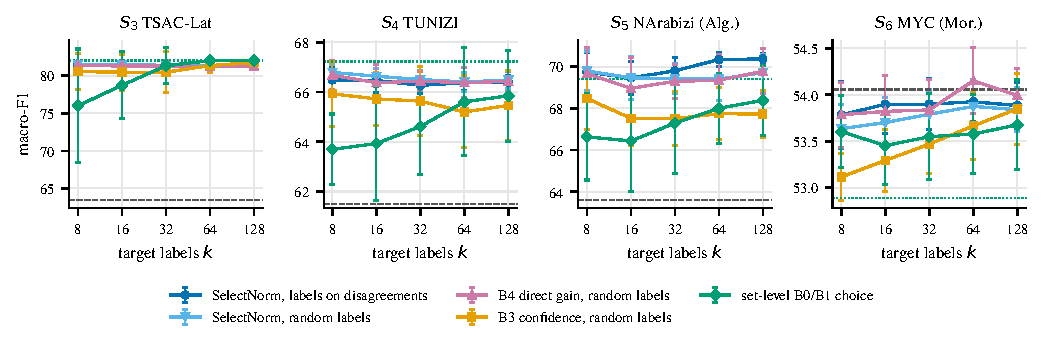
\includegraphics[width=\textwidth]{figures/fewlabel.pdf}
\caption{Few-label adaptation (mE5): macro-F1 against the number $k$ of labelled target sentences (5 draws $\times$ 5 seeds; error bars: s.d.). Dashed: B0; dotted: B1. ``Set-level choice'' picks B0 or B1 by accuracy on the $k$ labels.}
\label{fig:fewlabel}
\end{figure*}
With $k$ labelled target sentences, re-estimating the scalar shift of $\hat\rho$ changes macro-F1 relative to zero-shot SelectNorm-adapt with the same threshold by $-1.4$ to $+1.5$ points across encoders, regimes, sets and $k$ (mean $-0.01$; \cref{fig:fewlabel}). Spending the labels on disagreements, which \cref{prop:efficiency} shows to be $1/P(D{=}1)$ times more informative about the shift, makes little difference: averaged over encoders and sets, SelectNorm with targeted labels is between $-0.1$ and $+0.2$ points from SelectNorm with random labels at every $k$ (descriptive; not tested). In the Arabic-script regime, SelectNorm is clearly better than a set-level choice between B0 and B1 when $k\le 16$ (by 2.6--2.9 points on average), and the advantage shrinks to 0.3 points at $k=128$, consistent with M2: most of the usable signal is set-level.

\subsection{Normalizer, consistency and classifier regime}
\paragraph{Safeguards.} The safeguards of $T_{\rm cons}$ matter more than routing: always normalizing with $T_{\rm lex}$ or $T_{\rm rule}$ instead loses 4--11 points on every set for mE5, and routing over those normalizers recovers only part of the loss (\cref{tab:ablation}). Keeping out-of-lexicon tokens in Latin script ($T_{\rm cov}$) reduces disagreements by about a third and makes routing nearly irrelevant; it is worse than $T_{\rm cons}$ on the Tunisian sets and slightly better on $S_5$ and $S_6$.

\paragraph{Consistency with human transliteration (RQ4).} On NArabizi, B1 agrees with the prediction that $f$ makes on the human Arabic-script version of the same sentence for 73--77\% of inputs, against 61--67\% for B0 and 73--76\% for SelectNorm-adapt, so routing does not increase agreement further; $f$ itself reaches 65--77 macro-F1 on the human transliterations (per-encoder values in the released \texttt{consistency.csv}).

\paragraph{Classifier trained on both scripts.} When $f$ also sees synthetic Latin renderings (\textsc{+syn}, \cref{tab:main-syn}), the original view improves and the two views become more complementary: the oracle headroom stays similar, the win rate on disagreements moves towards 50\%, and SelectNorm-adapt exceeds the better single view in several cells. Against that view it is relevantly better once with Holm correction (MARBERTv2, $S_4$, $+1.1$) and twice more under the protocol's unadjusted criterion (mE5, $S_3$ $+2.1$, $S_4$ $+1.4$), and relevantly worse in two MYC cells under both (LaBSE $-2.4$, MARBERTv2 $-1.8$). Confidence thresholding and the ensemble share the gains; SelectNorm is never significantly better than B4 (worse once, $-0.4$).

\section{Discussion}
\label{sec:discussion}

\paragraph{What the factorization shows.}
A per-input router can fail because it cannot tell \emph{whether} the views disagree, \emph{which} wins when they do, how the latter shifts across domains, or because the apparent headroom is not real; measured separately, these have different weights here. Disagreement is moderately predictable (M1). Transfer matters in specific cells: for XLM-R on Algerian and Moroccan text, source $\hat\rho$ ranks direction at or below chance, and fitting it on the target turns a loss of up to 3.3 points into a small gain. But even fitted on the target, $\hat\rho$ gains at most 2.8 points over the best view in any cell (M2, M3). In our measurements the main limit is that the decision-point features say little about which view is right, even in domain, and a sizeable part of the oracle headroom is of the size that two classifiers differing only in their training sample also show (M4; a diagnostic reference, not a decomposition). The richer variants we tried did not change this (16 embedding components: $-1.2$ to $+1.1$ points, no consistent sign; gradient boosting, mE5 only: $-0.6$ to $+0.7$). These are limits of the features and estimators we evaluated; features computed after the second pass, fine-tuned representations or other estimators might do better, and our results do not show that the conditional advantage is intrinsically unpredictable. The same measurements can be made for other two-view choices with a frozen model, such as test-time augmentation or translate-test; we have not done so. Where oracle headroom is reported, a bootstrap-classifier reference helps to judge how much of it is classifier variability.

\paragraph{Where the signal is.}
The win rate on disagreements varies far more between encoder--dialect pairs (33--77\%) than our features resolve within a set, and on MYC every linguistic condition changes sign with the encoder. The useful decision is thus mostly set-level, which few labels resolve: with 64--128 target labels a set-level choice is on average within 0.3--0.7 points of SelectNorm with the same labels (descriptive). Targeted labels estimate the shift more efficiently (\cref{prop:efficiency}) but cannot fix a weak ranking.

\paragraph{Practical recommendations.}
For Arabizi with a frozen encoder, a linear head trained on Arabic script, and binary sentiment, our results suggest: (i) invest in normalizer safeguards first, since they matter more than routing (\cref{tab:ablation}); (ii) choose between normalizing and not at the level of a corpus or dialect, with on the order of a hundred labels; (iii) do not expect per-input routing that reads the first pass to save compute, except relative to running both views; (iv) when the classifier is trained on both scripts, learned routers, confidence thresholding or an ensemble sometimes gain a little over the better view, but can also lose on MYC.

\paragraph{Relation to prior findings.}
That transliteration helps unseen scripts on average is known \citep{muller2021unseen,moosa2023transliteration}; our results agree for Tunisian and Algerian Arabizi and add that the sign flips with the encoder on Moroccan text. Loss predictors for test-time transformations \citep{kim2020learningloss} and post-hoc deferral \citep{jitkrittum2023cascade} are the closest methods; SelectNorm is within one point of the direct-gain router in every cell, and the factorization adds a diagnosis, not an accuracy gain.

\section*{Limitations}
\textbf{Scope of the task.} All experiments use binary sentiment, where the factorization is exact with $\rho$ alone; the $K$-class form needs two conditional win rates. \textbf{Classifiers and scope.} Encoders are frozen and heads are linear; all conclusions are restricted to this setting. A fine-tuned encoder could change how often normalization helps and how predictable the winning view is; we did not fine-tune (CPU only), and the exploratory \textsc{+syn} regime is only a partial probe. \textbf{Normalizer.} $T$ is built from Tunisian resources (TArC lexicon, Tunisian digit conventions such as \textit{8}=\ar{ه}); its intrinsic accuracy is lower on Algerian NArabizi, and no Moroccan transliteration gold was available, so its validity on MYC is unmeasured. Safeguards were tuned on the TArC held-out split, and no independent transliteration test set was available, so intrinsic accuracy is not independently validated. \textbf{Data.} Cross-corpus differences mix dialect with platform, topic, period and label distribution; we do not attribute them to dialect alone. TUNIZI, NArabizi and MYC state no licence and MARBERTv2 has none on its model card; we use them for research only and do not redistribute them. \textbf{Development.} The pipeline was first exercised with a character n-gram classifier whose test results we inspected; this motivated the few-label setting. Pre-specified and exploratory analyses are distinguished in \cref{sec:setup}. \textbf{Analysis.} Mechanism intervals cover resampling of test sentences, not refitting of the estimators; the target-label ceiling uses linear $\hat\rho$ on the same features, so a richer model could find more signal. Features computed after $f(T(x))$ might predict direction better but need the second pass on every input; we did not study them. Equivalence statements use 95\% intervals against the protocol's 1-point margin, are post hoc and are not corrected for multiplicity. \textbf{Costs.} Per-sentence costs are estimated from a token-length model and checked by end-to-end timing of the deployed pipeline on 200 sentences per set, on one 4-core CPU without a GPU; relative costs on accelerators differ, especially for short inputs.


\bibliography{references}

\appendix
\small
\begin{table}[!htb]
\centering\footnotesize\setlength{\tabcolsep}{3pt}
\begin{tabular}{@{}lrrrr@{}}\toprule
Variant & $S_3$ & $S_4$ & $S_5$ & $S_6$\\\midrule
SelectNorm-adapt (full) & 81.3 & 66.9 & 69.8 & 53.7\\
\quad -- target re-estimation of $\hat\pi$ & 81.3 & 67.0 & 70.0 & 53.7\\
\quad Bayes threshold instead of tuned & 81.4 & 66.9 & 69.6 & 53.5\\
\quad $2\hat\rho-1$ only (no $\hat\pi$) & 81.3 & 66.9 & 69.8 & 53.6\\
\quad $\hat\pi$ only, tuned (label-free ranking) & 81.9 & 67.2 & 69.5 & 53.1\\
\quad confidence features only & 82.0 & 67.2 & 69.4 & 53.0\\
\quad -- confidence features & 81.5 & 66.9 & 69.6 & 53.6\\
\quad -- script features & 81.6 & 67.1 & 69.8 & 53.4\\
\quad -- normalizer reliability & 82.0 & 67.0 & 69.4 & 53.2\\
\quad + embedding PCA & 82.0 & 67.2 & 70.9 & 53.8\\
\quad gradient boosting & 82.0 & 67.1 & 69.6 & 53.1\\
\quad $T_{\rm lex}$ (no safeguards) & 80.7 & 64.6 & 65.2 & 53.0\\
\quad always $T_{\rm lex}$ & 77.8 & 61.8 & 63.2 & 47.9\\
\quad $T_{\rm rule}$ & 76.7 & 61.8 & 61.4 & 53.3\\
\quad always $T_{\rm rule}$ & 75.1 & 58.8 & 58.8 & 47.7\\
\quad $T_{\rm cov}$ (unknown tokens kept Latin) & 75.0 & 65.7 & 70.8 & 54.1\\
\quad always $T_{\rm cov}$ & 75.0 & 65.8 & 70.7 & 54.0\\
\bottomrule\end{tabular}

\caption{Ablations (mE5, $\lambda=0$, macro-F1, mean of five seeds). Rows with ``always'' are B1 with that normalizer.}
\label{tab:ablation}
\end{table}
\begin{table}[!htb]
\centering\footnotesize\setlength{\tabcolsep}{2.5pt}
\resizebox{\columnwidth}{!}{\begin{tabular}{@{}lrrrrr@{}}\toprule
 & \multicolumn{3}{c}{TArC development split (Tunisian)} & \multicolumn{2}{c}{NArabizi (Algerian, out of dialect)}\\\cmidrule(lr){2-4}\cmidrule(lr){5-6}
Strategy & Word acc. & Foreign kept (P/R) & Negation & Word acc. & Foreign kept (P/R)\\\midrule
$T_{\rm rule}$ & 36.3 & --/0 & 29.1 & 39.0 & --/0\\
$T_{\rm lex}$ & 69.5 & --/0 & 54.4 & 47.6 & --/0\\
$T_{\rm cons}$ & 69.1 & 96/79 & 96.1 & 46.8 & 93/53\\
\bottomrule\end{tabular}
}
\caption{Normalizer accuracy against human Arabic-script transliterations: \emph{development} results, not an independent test. TArC: 20\% of sentences, not used for the lexicon $\mathcal L$ but used to design the safeguards. NArabizi: whole corpus, nothing fitted to it, but scored during development. ``Foreign kept'': precision/recall of keeping annotated French/English tokens in Latin script; negation: accuracy on circumfix-negated verbs. Audit: no hand-listed word occurs only in the development split; on the 87\% of tokens no rule touches, word accuracy is 65.8\%; with the splits' roles swapped, negation is kept in 94.4\% and foreign precision/recall is 95/77.}
\label{tab:intrinsic}
\end{table}
\begin{table*}[t]
\centering\scriptsize\setlength{\tabcolsep}{3pt}
\begin{tabular}{@{}llrrrr@{}}\toprule
Enc. & Set & vs.\ B1 & vs.\ B3 & vs.\ B4 & vs.\ SN-src\\\midrule
mE5 & $S_3$ & -0.71 \scriptsize[-1.25, -0.21] & -0.67 \scriptsize[-1.21, -0.17] & -0.07 \scriptsize[-0.27, +0.13]$^{\dagger}$ & -0.03 \scriptsize[-0.11, +0.06]$^{\dagger}$\\
 & $S_4$ & -0.31 \scriptsize[-0.80, +0.17]$^{\dagger}$ & -0.23 \scriptsize[-0.72, +0.25]$^{\dagger}$ & -0.03 \scriptsize[-0.25, +0.18]$^{\dagger}$ & -0.04 \scriptsize[-0.16, +0.08]$^{\dagger}$\\
 & $S_5$ & +0.39 \scriptsize[-0.22, +1.01] & +0.39 \scriptsize[-0.22, +1.01] & -0.14 \scriptsize[-0.57, +0.28]$^{\dagger}$ & -0.17 \scriptsize[-0.47, +0.11]$^{\dagger}$\\
 & $S_6$ & +0.76 \scriptsize[+0.23, +1.30] & +0.75 \scriptsize[+0.23, +1.29] & +0.02 \scriptsize[-0.22, +0.27]$^{\dagger}$ & -0.04 \scriptsize[-0.18, +0.11]$^{\dagger}$\\
\midrule
XLM-R & $S_3$ & +0.99 \scriptsize[+0.01, +2.02] & +0.91 \scriptsize[-0.07, +1.91] & +0.28 \scriptsize[+0.04, +0.52]$^{\dagger}$ & +0.07 \scriptsize[-0.02, +0.17]$^{\dagger}$\\
 & $S_4$ & -0.66 \scriptsize[-1.20, -0.11] & -0.60 \scriptsize[-1.14, -0.04] & -0.04 \scriptsize[-0.18, +0.10]$^{\dagger}$ & +0.02 \scriptsize[-0.04, +0.09]$^{\dagger}$\\
 & $S_5$ & -0.01 \scriptsize[-0.42, +0.45]$^{\dagger}$ & +0.09 \scriptsize[-0.34, +0.56]$^{\dagger}$ & -0.18 \scriptsize[-0.41, +0.03]$^{\dagger}$ & -0.25 \scriptsize[-0.45, -0.07]$^{*}$$^{\dagger}$\\
 & $S_6$ & -3.76 \scriptsize[-4.58, -2.93]$^{*}$ & -3.77 \scriptsize[-4.58, -2.94]$^{*}$ & -0.23 \scriptsize[-0.42, -0.03]$^{\dagger}$ & +0.53 \scriptsize[+0.33, +0.73]$^{*}$$^{\dagger}$\\
\midrule
LaBSE & $S_3$ & -0.19 \scriptsize[-0.75, +0.35]$^{\dagger}$ & -0.24 \scriptsize[-0.73, +0.23]$^{\dagger}$ & +0.03 \scriptsize[-0.19, +0.24]$^{\dagger}$ & +0.03 \scriptsize[-0.08, +0.14]$^{\dagger}$\\
 & $S_4$ & -0.37 \scriptsize[-1.01, +0.28] & -0.35 \scriptsize[-0.95, +0.25]$^{\dagger}$ & +0.15 \scriptsize[-0.06, +0.34]$^{\dagger}$ & +0.01 \scriptsize[-0.11, +0.14]$^{\dagger}$\\
 & $S_5$ & +0.62 \scriptsize[-1.20, +2.44] & +0.57 \scriptsize[-1.17, +2.32] & -0.07 \scriptsize[-0.60, +0.47]$^{\dagger}$ & +0.34 \scriptsize[-0.01, +0.71]$^{\dagger}$\\
 & $S_6$ & +5.46 \scriptsize[+4.44, +6.50]$^{*}$ & +5.04 \scriptsize[+4.05, +6.04]$^{*}$ & +0.32 \scriptsize[+0.06, +0.58]$^{\dagger}$ & +0.54 \scriptsize[+0.30, +0.79]$^{*}$$^{\dagger}$\\
\midrule
MARBERTv2 & $S_3$ & -0.01 \scriptsize[-0.65, +0.64]$^{\dagger}$ & -0.16 \scriptsize[-0.77, +0.48]$^{\dagger}$ & +0.03 \scriptsize[-0.18, +0.23]$^{\dagger}$ & -0.09 \scriptsize[-0.20, +0.01]$^{\dagger}$\\
 & $S_4$ & +0.57 \scriptsize[+0.08, +1.06] & +0.16 \scriptsize[-0.37, +0.68]$^{\dagger}$ & +0.06 \scriptsize[-0.10, +0.22]$^{\dagger}$ & +0.00 \scriptsize[-0.07, +0.08]$^{\dagger}$\\
 & $S_5$ & +0.58 \scriptsize[-0.45, +1.64] & +0.58 \scriptsize[-0.45, +1.64] & -0.11 \scriptsize[-0.63, +0.40]$^{\dagger}$ & -0.01 \scriptsize[-0.36, +0.35]$^{\dagger}$\\
 & $S_6$ & -0.53 \scriptsize[-1.15, +0.08] & -0.61 \scriptsize[-1.22, -0.01] & +0.12 \scriptsize[-0.19, +0.43]$^{\dagger}$ & -0.01 \scriptsize[-0.15, +0.12]$^{\dagger}$\\
\bottomrule\end{tabular}

\caption{Paired differences in macro-F1 (SelectNorm-adapt minus baseline, $\lambda=0$, seed-averaged) with 95\% paired-bootstrap intervals (10{,}000 resamples of test sentences). $^{*}$: Holm-corrected $p<0.05$ over the protocol's 20 comparisons per encoder. $^{\dagger}$: the interval lies inside $(-1,+1)$, the protocol's relevance margin; reading this as equivalence is post hoc and not corrected for multiplicity. Intervals without either mark are inconclusive about both difference and equivalence.}
\label{tab:paired}
\vspace{2mm}
\centering\scriptsize\setlength{\tabcolsep}{3.5pt}
\begin{tabular}{@{}lrrrrrrrr@{}}\toprule
 & \multicolumn{4}{c}{\textbf{mE5+syn}} & \multicolumn{4}{c}{\textbf{XLM-R+syn}}\\
\cmidrule(lr){2-5}\cmidrule(lr){6-9}
 & $S_3$ & $S_4$ & $S_5$ & $S_6$ & $S_3$ & $S_4$ & $S_5$ & $S_6$\\\midrule
B0 original & 80.9$^{\triangledown}$ & 65.6$^{\triangledown}$ & 69.1 & \textbf{61.5} & 69.0$^{\triangledown}$ & 59.8$^{\triangledown}$ & 64.7 & 59.7\\
B1 always normalize & 81.6 & 67.5 & 72.6 & 58.0$^{\triangledown}$ & 72.8 & 63.2 & 62.9 & 59.1\\
B2 random, matched rate & 81.2 & 66.5 & 70.4 & 61.0 & 70.8 & 61.6 & 63.9 & 59.7\\
B3 confidence threshold & 83.0 & 68.7 & \textbf{73.2} & 60.7 & 74.5 & 63.0 & 64.7 & 60.3\\
B4 direct gain & \textbf{83.8} & \textbf{68.9} & 72.4 & 60.9 & \textbf{74.5} & 63.8 & 65.1 & 60.6\\
B4b per-view loss & 83.8 & 68.9 & 72.5 & 60.8 & 74.3 & 63.8 & 65.0 & 60.5\\
SelectNorm-src & 83.6 & 68.8 & 72.9 & 61.1 & 74.3 & 63.5 & \textbf{65.5} & 60.4$^{\triangledown}$\\
\rowcolor{black!6}SelectNorm-adapt & 83.7 & 68.9 & 73.0 & 61.1 & 74.3 & 63.5 & 65.4 & 60.6\\
\quad Bayes threshold $\lambda\bar c$ & 83.7 & 68.8 & 73.2 & 61.1 & 74.5 & \textbf{63.9} & 65.0 & \textbf{60.8}\\
\addlinespace[2pt]
R two-view ensemble$^\dagger$ & 83.7 & 68.9 & 74.7 & 60.5 & 75.8 & 64.0 & 65.6 & 60.7\\
B6 oracle$^\ddagger$ & 91.7 & 80.9 & 85.7 & 71.4 & 86.3 & 79.0 & 80.6 & 73.5\\
\midrule[\heavyrulewidth]
 & \multicolumn{4}{c}{\textbf{LaBSE+syn}} & \multicolumn{4}{c}{\textbf{MARBERTv2+syn}}\\
\cmidrule(lr){2-5}\cmidrule(lr){6-9}
 & $S_3$ & $S_4$ & $S_5$ & $S_6$ & $S_3$ & $S_4$ & $S_5$ & $S_6$\\\midrule
B0 original & 76.6$^{\triangledown}$ & 64.9$^{\triangledown}$ & 71.3 & \textbf{62.4}$^{\blacktriangle}$ & 77.0$^{\triangledown}$ & 64.2$^{\triangledown}$ & 57.0 & 50.1$^{\triangledown}$\\
B1 always normalize & 83.7 & 67.8 & 74.3 & 58.7$^{\triangledown}$ & 81.8 & 67.8$^{\triangledown}$ & 59.3 & \textbf{60.7}$^{\blacktriangle}$\\
B2 random, matched rate & 80.3 & 66.3 & 72.9 & 59.9 & 80.8 & 67.3 & 59.1 & 58.3\\
B3 confidence threshold & \textbf{84.3} & 68.2 & 74.3 & 60.4 & 82.9 & 68.7 & 59.3 & 59.5$^{\blacktriangle}$\\
B4 direct gain & 84.3 & \textbf{68.5} & 74.4 & 59.7 & 82.5 & 68.7 & 59.6 & 59.3$^{\blacktriangle}$\\
B4b per-view loss & 84.1 & 68.5 & \textbf{74.8} & 59.6 & 82.3 & 68.7 & 59.6 & 58.7\\
SelectNorm-src & 84.1 & 68.3 & 74.7 & 60.0 & 82.5 & 68.8 & 59.8 & 59.0\\
\rowcolor{black!6}SelectNorm-adapt & 84.2 & 68.2 & 74.6 & 60.0 & 82.6 & 68.9 & \textbf{59.9} & 58.9\\
\quad Bayes threshold $\lambda\bar c$ & 84.2 & 68.2 & 74.8 & 60.1 & \textbf{83.0} & \textbf{69.2} & 59.8 & 58.6\\
\addlinespace[2pt]
R two-view ensemble$^\dagger$ & 83.5 & 68.8 & 76.6 & 61.3 & 83.6 & 69.0 & 59.3 & 57.3\\
B6 oracle$^\ddagger$ & 92.9 & 81.1 & 86.8 & 73.1 & 92.6 & 81.6 & 72.3 & 69.3\\
\bottomrule\end{tabular}

\caption{As \cref{tab:main}, with $f$ also trained on synthetic Latin renderings (\textsc{+syn}, exploratory regime).}
\label{tab:main-syn}
\end{table*}
\begin{table*}[t]
\centering\footnotesize\setlength{\tabcolsep}{3pt}
\resizebox{\textwidth}{!}{\begin{tabular}{@{}lrrrrrrrrrrrrrrrr@{}}\toprule
 & \multicolumn{4}{c}{$S_3$ \scriptsize(help 376, harm 114)} & \multicolumn{4}{c}{$S_4$ \scriptsize(help 538, harm 402)} & \multicolumn{4}{c}{$S_5$ \scriptsize(help 124, harm 89)} & \multicolumn{4}{c}{$S_6$ \scriptsize(help 407, harm 456)}\\\cmidrule(lr){2-5}\cmidrule(lr){6-9}\cmidrule(lr){10-13}\cmidrule(lr){14-17}
System & Sel.\,\% & Harm & Capt.\,\% & Cost & Sel.\,\% & Harm & Capt.\,\% & Cost & Sel.\,\% & Harm & Capt.\,\% & Cost & Sel.\,\% & Harm & Capt.\,\% & Cost\\\midrule
B1 & 100.0 & 8.0 & 100.0 & 0.98 & 100.0 & 14.0 & 100.0 & 0.97 & 100.0 & 12.2 & 100.0 & 0.98 & 100.0 & 10.9 & 100.0 & 1.04\\
B3 & 98.9 & 8.0 & 99.7 & 1.97 & 99.1 & 14.0 & 99.5 & 1.97 & 99.5 & 12.2 & 100.0 & 1.97 & 98.5 & 10.9 & 99.9 & 2.03\\
B4 & 90.2 & 7.6 & 96.1 & 1.89 & 88.8 & 13.1 & 93.8 & 1.87 & 86.4 & 10.9 & 95.5 & 1.84 & 66.8 & 7.9 & 76.9 & 1.70\\
SN-adapt & 89.0 & 7.6 & 95.7 & 1.88 & 87.0 & 13.0 & 93.3 & 1.86 & 85.7 & 11.3 & 96.8 & 1.83 & 65.9 & 8.3 & 80.9 & 1.69\\
Oracle & 26.4 & 0.0 & 100.0 & 1.26 & 18.7 & 0.0 & 100.0 & 1.18 & 17.0 & 0.0 & 100.0 & 1.17 & 9.7 & 0.0 & 100.0 & 1.10\\
\bottomrule\end{tabular}
}
\caption{Routing behaviour (mE5, $\lambda=0$): selection rate, harmful transformations per 100 inputs, share of oracle opportunities captured, and estimated cost relative to B0 (\cref{app:repro}). Help/harm: number of inputs where normalization corrects/introduces an error.}
\label{tab:routing}
\vspace{2mm}
\centering\scriptsize\setlength{\tabcolsep}{4pt}
\begin{tabular}{@{}llllllll@{}}\toprule
Enc. & Set & AUC$_\pi$ & AUC$_\rho$ & AUC$_\rho^{\rm tgt}$ & gap (pts) & $\Delta_{\rm src}$ & $\Delta_{\rm tgt}$\\\midrule
mE5 & $S_3$ & [0.65, 0.71] & [0.60, 0.72] & [0.58, 0.69] & [-0.8, +6.8] & [-1.0, -0.2] & [-0.8, +0.7]\\
 & $S_4$ & [0.62, 0.66] & [0.52, 0.60] & [0.54, 0.61] & [+15.2, +21.9] & [-0.8, +0.1] & [-1.2, +1.0]\\
 & $S_5$ & [0.57, 0.66] & [0.55, 0.71] & [0.49, 0.64] & [+7.7, +21.1] & [-0.2, +0.5] & [-1.5, +2.9]\\
 & $S_6$ & [0.73, 0.76] & [0.50, 0.57] & [0.52, 0.60] & [+16.7, +23.5] & [-1.7, +0.6] & [-0.7, +0.9]\\
\midrule
XLM-R & $S_3$ & [0.61, 0.67] & [0.66, 0.76] & [0.63, 0.73] & [-0.8, +6.2] & [+0.1, +2.0] & [-0.3, +2.0]\\
 & $S_4$ & [0.64, 0.68] & [0.53, 0.60] & [0.53, 0.61] & [+8.0, +14.6] & [-0.9, +0.0] & [-0.2, +0.8]\\
 & $S_5$ & [0.65, 0.74] & [0.35, 0.53] & [0.50, 0.69] & [+4.5, +18.0] & [+0.0, +0.7] & [-2.1, +0.8]\\
 & $S_6$ & [0.71, 0.74] & [0.41, 0.48] & [0.63, 0.70] & [-10.9, -4.7] & [-4.0, -2.5] & [+0.6, +1.7]\\
\midrule
LaBSE & $S_3$ & [0.66, 0.72] & [0.55, 0.67] & [0.47, 0.60] & [-4.5, +3.7] & [-0.4, +0.6] & [-0.6, +0.3]\\
 & $S_4$ & [0.63, 0.67] & [0.54, 0.61] & [0.55, 0.62] & [+3.0, +8.9] & [-1.0, +0.2] & [-1.2, +0.3]\\
 & $S_5$ & [0.61, 0.69] & [0.52, 0.66] & [0.48, 0.62] & [-2.9, +9.6] & [-1.3, +2.1] & [-2.0, +2.4]\\
 & $S_6$ & [0.67, 0.70] & [0.54, 0.60] & [0.61, 0.68] & [+13.0, +18.5] & [-3.8, -1.3] & [+0.2, +1.3]\\
\midrule
MARBERTv2 & $S_3$ & [0.66, 0.72] & [0.59, 0.69] & [0.55, 0.66] & [-2.2, +5.3] & [-0.4, +0.6] & [-1.2, +0.5]\\
 & $S_4$ & [0.69, 0.73] & [0.58, 0.65] & [0.61, 0.68] & [+10.0, +15.7] & [-0.1, +0.9] & [+1.6, +3.9]\\
 & $S_5$ & [0.70, 0.77] & [0.55, 0.69] & [0.47, 0.62] & [+7.0, +19.8] & [-1.9, +1.2] & [-1.3, +2.9]\\
 & $S_6$ & [0.69, 0.72] & [0.52, 0.58] & [0.59, 0.66] & [+1.7, +7.1] & [-0.9, +0.3] & [+0.3, +1.8]\\
\bottomrule\end{tabular}

\caption{95\% intervals for the mechanism measurements of \cref{tab:mechanism} (1{,}000 bootstrap resamples of test sentences, seed-averaged within each resample; estimators not refitted).}
\label{tab:mechanism-ci}
\vspace{2mm}
\centering\scriptsize\setlength{\tabcolsep}{3pt}
\begin{tabular}{@{}lrrrrrr@{}}\toprule
 & views & \multicolumn{5}{c}{reference headroom (two resampled classifiers)}\\
\cmidrule(lr){3-7}
Enc. & headroom & bootstrap & 80\% sub. & 50\% sub. & boot., $3C$ & boot., $C/3$\\\midrule
mE5 & 8.0--14.1 & 6.1--9.1 & 2.9--4.0 & 4.8--6.8 & 8.0--10.9 & 4.2--7.3\\
XLM-R & 7.3--10.7 & 3.4--5.1 & 2.1--3.0 & 1.7--3.6 & 5.1--7.2 & 2.0--4.2\\
LaBSE & 7.9--14.9 & 6.6--7.4 & 3.3--3.9 & 6.1--7.0 & 7.2--8.6 & 5.4--6.2\\
MARBERTv2 & 11.5--16.5 & 10.6--15.3 & 4.7--6.3 & 9.4--14.5 & 14.8--21.9 & 8.2--11.3\\
\bottomrule\end{tabular}

\caption{Sensitivity of the oracle reference (range over the four sets). ``Views headroom'': oracle over $x$ and $T(x)$ minus the best view; other columns: the same for two classifiers differing only in their training sample (bootstrap as in \cref{tab:mechanism}, 80\%/50\% subsamples, or bootstrap with $C\times3$ or $C/3$), applied to $x$; mean of 10 pairs.}
\label{tab:noise}
\end{table*}
\section{Proofs}
\label{app:proofs}

\paragraph{Bayes rule (\cref{eq:bayes}).}
For fixed $z$, the conditional risk of $g(z)=a$ is $\mathbb E[e_a\mid z]+\lambda\,\mathbb E[c_0+c_T\mid z]+\lambda\bar c(z)\,a$, where the middle term does not depend on $a$. Choosing $a=1$ is strictly better iff $\mathbb E[e_1\mid z]+\lambda\bar c(z)<\mathbb E[e_0\mid z]$, i.e.\ $B(z)>\lambda\bar c(z)$. Minimizing pointwise minimizes \cref{eq:risk}. \qed

\paragraph{Factorization (\cref{eq:factor}).}
If $D=0$ then $\hat y_0=\hat y_1$ and $e_0=e_1$, so $e_0-e_1=D(e_0-e_1)$. If $D=1$ and $y\in\{0,1\}$, then $\hat y_0=1-\hat y_1$, hence $e_0=W$ and $e_1=1-W$, and $e_0-e_1=2W-1$. Therefore $B(z)=\mathbb E[D(2W-1)\mid z]=P(D{=}1\mid z)\,\big(2P(W{=}1\mid D{=}1,z)-1\big)$. For $K$ classes, $e_0-e_1=D\big(\mathbf 1[\hat y_1{=}y]-\mathbf 1[\hat y_0{=}y]\big)$, which gives $\pi(\rho_1-\rho_0)$. \qed

\paragraph{\Cref{prop:regret}.}
For any $z$, if $\hat g(z)=g^\star(z)$ the conditional excess risk is zero. Otherwise it equals $|B(z)-\lambda\bar c(z)|$, and since $\hat B-\lambda\bar c$ and $B-\lambda\bar c$ have different signs (or $\hat B=\lambda\bar c$), $|B-\lambda\bar c|\le|\hat B-B|$. Taking expectations gives $R(\hat g)-R(g^\star)\le\mathbb E|\hat B-B|$. Writing $\hat B-B=\hat\pi(2\hat\rho-1)-\pi(2\rho-1)=(\hat\pi-\pi)(2\rho-1)+2\hat\pi(\hat\rho-\rho)$ and applying the triangle inequality concludes. \qed

\paragraph{\Cref{prop:efficiency}.}
Write $r_i=\operatorname{logit}\hat\rho(z_i)$ and $q_i=\sigma(r_i+b)$. A labelled target example contributes the log-likelihood $D_i\big[W_i\log q_i+(1-W_i)\log(1-q_i)\big]$: when $D_i=0$ the label is uninformative about $b$ because $e_0=e_1$ regardless of $y_i$, and the model of $W$ is defined only on disagreements. The per-example Fisher information about $b$ is $D_i\,q_i(1-q_i)$. Under random sampling from $Q$, its expectation is $P_Q(D{=}1)\,\mathbb E_Q[q(1-q)\mid D{=}1]$; under sampling from $Q(\cdot\mid D{=}1)$, which is possible without labels because $D$ is observable, it is $\mathbb E_Q[q(1-q)\mid D{=}1]$. Information is additive over independent draws, so the ratio is $1/P_Q(D{=}1)$. \qed

The proposition concerns the scalar shift only. It does not claim that a shifted $\hat\rho$ recovers the target-optimal rule; that depends on whether the shift is close to a constant in logit space, which the experiments test.






\section{Reproducibility}
\label{app:repro}
\paragraph{Encoders and software.} Encoders are loaded at pinned revisions with SHA-256-verified weights: XLM-R base \texttt{e73636d} (MIT), mE5 base \texttt{d128750} (MIT), LaBSE \texttt{836121a} (Apache-2.0), MARBERTv2 \texttt{fe88db9} (no licence stated). Representations: mean of the last layer over non-padding tokens, at most 128 subwords, $\ell_2$-normalized; mE5 inputs carry \texttt{query:}. Python 3, scikit-learn 1.9.1, NumPy 2.5.3; code, configuration, logs and the protocol are released.

\paragraph{Classifier $f$.} $\ell_2$-regularized logistic regression; $C\in\{0.01,0.03,\ldots,100\}$ selected by macro-F1 on TSAC-\textsc{ar} dev; temperature fitted on the same split by NLL. The \textsc{+syn} regime adds the synthetic Latin rendering $G(x)$ of every training and dev sentence.

\paragraph{Router.} $\hat\pi,\hat\rho$: logistic regression on standardized $z$ ($C=1$); 17 features: confidence, margin and entropy of $p_0$ (\textsc{conf}); length, Latin and Arabic shares, digit-as-letter, emoji and upper-case rates (\textsc{script}); lexicon, rule-fallback, ambiguity, protected, negation, laughter and changed-token rates and lexicon entropy of $T$ (\textsc{trel}). Policy split 80/20 of TSAC-\textsc{lat} train with seed $1000+s$; the 20\% part tunes thresholds. 

\paragraph{Few-label audit.} \texttt{check\_fewlabel.py} replays every targeted and random label draw of all eight encoder--regime runs (8{,}000 draws), saves the sampled source identifiers, and counts any sampled label from the scored fold, any shared source identifier or normalized text between sampled and scored sentences, and any targeted sentence that is not a disagreement: none. A rerun of \texttt{adapt.py} for mE5 with index logging matches the replay in all 1{,}000 draws and the archived results in all 2{,}500 rows. In 375 targeted draws ($S_5$, $k{=}128$) fewer than $k$ disagreements were available.

\paragraph{Per-example exports.} \texttt{results/export/per\_example} gives, per encoder, regime and set, sentence and source identifiers, labels, both views' probabilities and every system's $\lambda{=}0$ prediction per seed. \texttt{scripts/reproduce\_stats.py} (NumPy and pandas only) recomputes from them every difference, interval and $p$-value of \cref{tab:main,tab:paired} for all four encoders exactly.

\paragraph{Mean vs input-dependent cost (exploratory).} Since $T(x)$ is known at the decision point, the token model also gives each input's own avoidable cost $c_1(x)$. Replacing $\lambda\bar c$ by $\lambda c_1(x)$ ($\lambda>0$, all encoders, sets, seeds) lowers cost by 0--0.11 passes and changes macro-F1 by $-2.0$ to $+0.6$ (means $-0.03$ and $-0.13$); it is no worse on both in 29 of 80 cells and trades accuracy for cost in 48: it moves along the frontier.

\paragraph{Costs.} $c_T$ is the measured normalizer time (about 0.4\% of a pass). $c_0,c_1$ are \emph{estimated} per sentence by a per-encoder model $a+b\cdot$tokens fitted to measured batch-1 latencies of 300 sentences per set and view (e.g.\ mE5 $a=19.6$\,ms, $b=0.32$\,ms/token, $R^2=0.68$), as used in \cref{fig:pareto,tab:routing}. \texttt{measured\_cost.py} runs the deployed pipeline on raw text at batch size 1 with nothing cached (pinned encoder, the trained head refitted deterministically, which reproduces the cached probabilities exactly, normalizer, features, each seed's router and $\lambda{=}0$ threshold, second pass only when selected). On all 9{,}220 test sentences, none of the 184{,}400 live routing decisions (4 encoders $\times$ 5 seeds) or final predictions differs from the archived ones (probabilities within $1.6\cdot10^{-4}$). Timed back to back on 200 sentences per set: B0 22--31\,ms; relative costs within $-0.02$ to $+0.05$ of the estimates for B1 and R, $+0.03$ to $+0.07$ for SelectNorm (features are not in the token model). mE5 was re-timed after a concurrent job overlapped it (both runs archived).


\end{document}
